\documentclass[letter, 11pt, onecolumn]{article}


\usepackage{geometry}
\geometry{letterpaper, margin=1in}
\usepackage{amsmath}
\usepackage{amssymb}  
\usepackage{amsthm}
\usepackage{ulem} 
\usepackage{graphicx}
\usepackage{subfig} 
\usepackage{hyperref}

\graphicspath{ {images/} }


\title{\vspace{-2.0cm}PH 481 Physical Optics: Lab 2 }
\author{John L Waczak \\ Lab Partner: Darlene Focht}
\date{\today}


\begin{document}
	\maketitle

\section*{Introduction} 
Lab 2 studies the phenomena of transmittance and reflectance. In particular, we looked at the interaction of laser light of multiple polarizations with dielectric materials such as glass and acrylic. The Brewster angle was found for P polarized light. Using this this angle, transmission and reflection coefficients were measured as a function of incident angle for both the P and S polarizations. Finally, we determined the index of refraction for a sample of acrylic by measuring the apparent beam separation at an incident angle of $\theta = \frac{\pi}{4}$ radians. 

\section*{Theory}
For large intensities light may be viewed as an electromagnetic wave propagating through space. In the case of lasers, we treat the light as a plane wave being emitted from a far away source. The general equation for an electromagnetic plane wave combined with the appropriate boundary conditions for dielectric media result in a set of equations that determine how light refracts from one material through another. They are called Fresnel's equations and they dictate how much light is transmitted through an interface versus how much is reflected (depending on the polarization). We let P represent parallel polarization and S perpendicular. Under this notation Fresnel's equations are: 
	\begin{align}
		r_s &= \frac{n_1\cos\theta_i+n_2\cos\theta_t}{n_i\cos\theta_1+n_2\cos\theta_t} \\ 
		t_s &= \frac{2n_1\cos\theta_i}{n_1\cos\theta_i+n_2\cos\theta_t} \\ 
		r_p &= \frac{n_2\cos\theta_i-n_1\cos\theta_t}{n_1\cos\theta_t+n_2\cos\theta_i} \\ 
		t_p &= \frac{2n_1\cos\theta_i}{n_1\cos\theta_t+n_2\cos\theta)1}
	\end{align}
Of course in our optics lab we do not directly measure the strength of the electric field but rather the intensity of laser light. In general intensity is proportional to the square of the electric field (time averaged) and so we can define R and T as the reflection and transmission coefficients for the intensity which we will be trying to match in our experiments. The only caveat is the because transmitted light is in a different medium $n_2$ we must consider how Snell's law of refraction impacts each of these quantities. This leads to the following set of equations: 
	\begin{align}
		R &= r^2 \\ 
		T &= \frac{n_2\cos\theta_t}{n1\cos\theta_i}t^2
	\end{align} 
Of particular importance is that when measuring the transmission in throughout this lab's experiments, light transmits first into the optical device and then transmits a second time back to air before any measurements are made. Thus the effective total Transmission is just the product of the transmission coefficients for each interface and is written as $T = T_{12}T_{21}$.\\ 

\noindent Another import physical phenomena is the zero reflection angle known as Brewster's angle. This is a special case where P polarized light goes to zero. This is expressed in the equation: 
	\begin{equation}
		\theta_B + \theta_t = \frac{\pi}{2}
	\end{equation} 
Asserting this requirement into Snell's law leads to: 
	\begin{align}
		n_1\sin(\theta_B) &= n_2\sin(\theta_B-\pi/2) \nonumber\\ 
		n_1\sin(\theta_B) &= n_2\cos(\theta_B) \nonumber\\ 
		\theta_B &= \arctan\Big(\frac{n_2}{n_1}\Big)
	\end{align}
For the first experiment, $n_1 \approx 1, n_2 = 1.5$. Plugging this in yields Brewster's angle at
	\begin{equation}
		\theta_B = \arctan(1.5) \approx 56.3^{\circ}
	\end{equation}
	
\section*{Experiment} 
In the first two experiments we were charged with finding the reflection and transmission functions for both P and S polarized light. First the laser was aligned using two mirrors and two irises in order to begin to construct the u-shape geometry shown in the following figure: 
	\begin{figure}[h!]
		\centering
		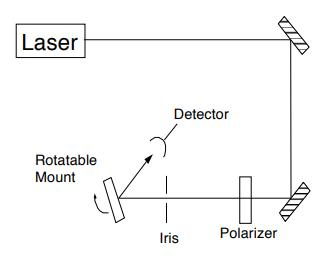
\includegraphics[width=0.45\columnwidth]{setup}
		\caption{U-shaped table geometry}
	\end{figure}
At the end of the optical rail a rotatable mount was placed to hold a piece of glass used to reflect the laser light. In order to ensure the light was in the p polarization, we angled the glass to $56.3^{\circ}$  in order to search for Brewster's angle. Once we found the dimmest angle by slightly adjusting the the glass, we inserted a polarizer into the beams path as shown in figure 1, adjusting it's setting until the reflected laser light disappeared. For our table this occurred at a polarizer setting of $160.5^{\circ}$. This defined the P polarization. Later to change the laser's state to S polarization this setting was shifted by 90 degrees to $70.5^{\circ}$. We measured $\theta_B = 56.8471^{\circ}$. Using this we can derive the index of refraction for the glass using (8). 
	\begin{equation}
		n_g = \tan(56.8471^{\circ}) = 1.53
	\end{equation}
	
\noindent After noting this value we set up the Thor Labs photodetector to a magnetic mount and connected it to an oscilloscope using a $43 k\Omega$ resistor. Then the reflection and transmission functions for the P polarization were determined by varying the angle and reading off the voltage. This value was normalized with the maximum photodetector voltage which we determined based on our resistor to be 11.1 volts. \\ 

\noindent Finally, we performed an experiment to determine the index of refraction of a 17mm thick piece of plexiglass (acrylic). To do this we set the incident angle of the slab to $\theta_i = 45^{\circ}$ and measured the displacement of the exiting beam from that of the $\theta_i = 0$ mark. 

\section*{Results} 
The following figures show our measured reflectance for each polarization (blue) plotted against the theoretical for the index of refraction determined in the first part of the lab. 
	\begin{center}
		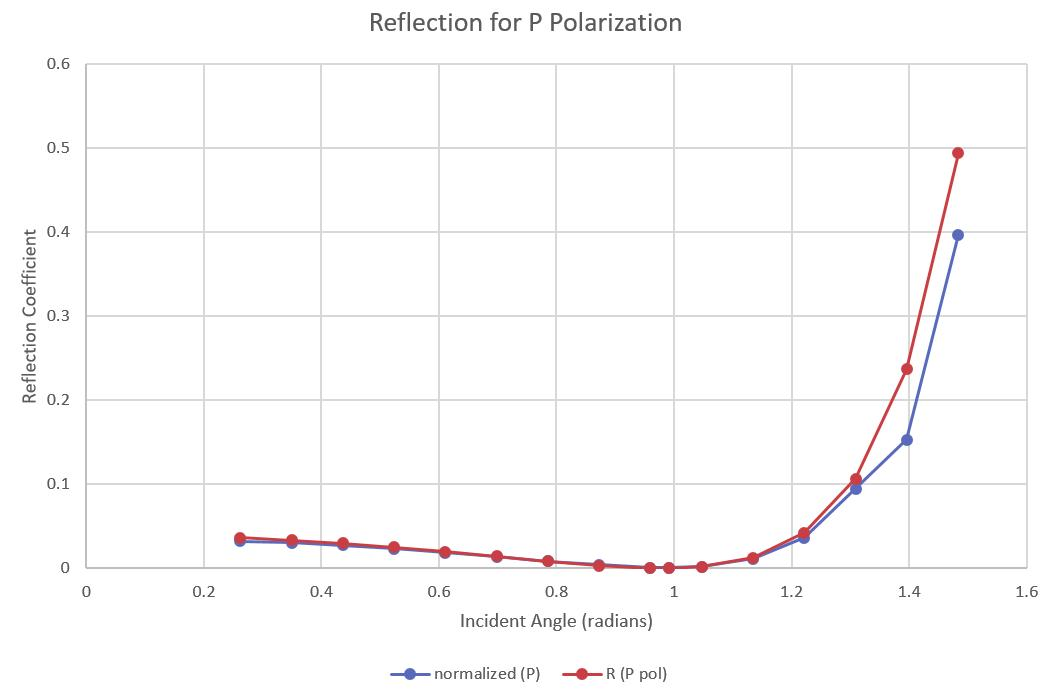
\includegraphics[width=0.75\columnwidth]{ref_p}\\
		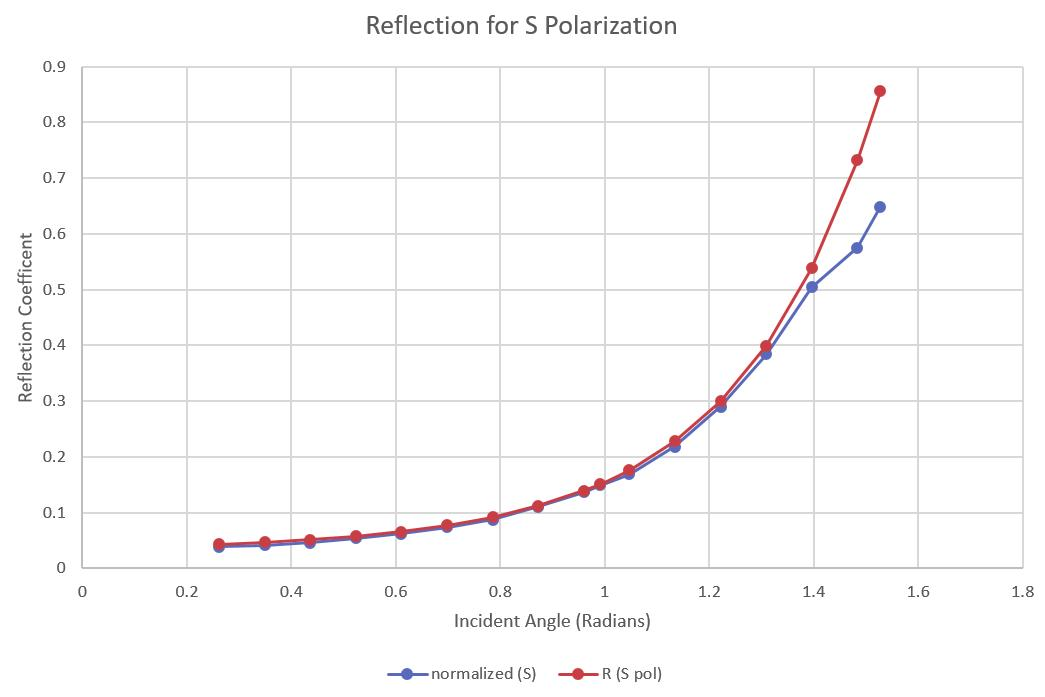
\includegraphics[width=0.75\columnwidth]{ref_s}
	\end{center} 
	
\noindent Similarly, for the transmission coefficients, the following figure illustrates each polarization compared with its theoretical curve based off of the Fresnel equations. Remember that for transmitted light we must consider the composition of two transmissions between each face of the glass slide. Thus our theoretical curves make use of $T = T_{12}\cdot T_{21}$ as mentioned above after eqn (6).\\ 
	\begin{center}
		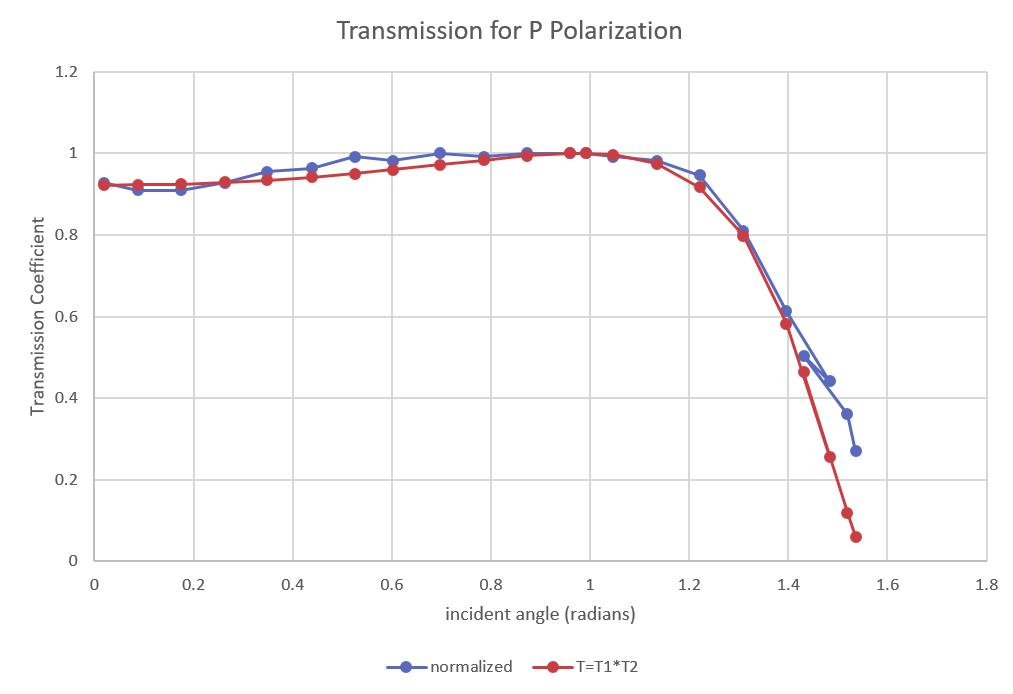
\includegraphics[width=0.75\columnwidth]{trans_p}\\
		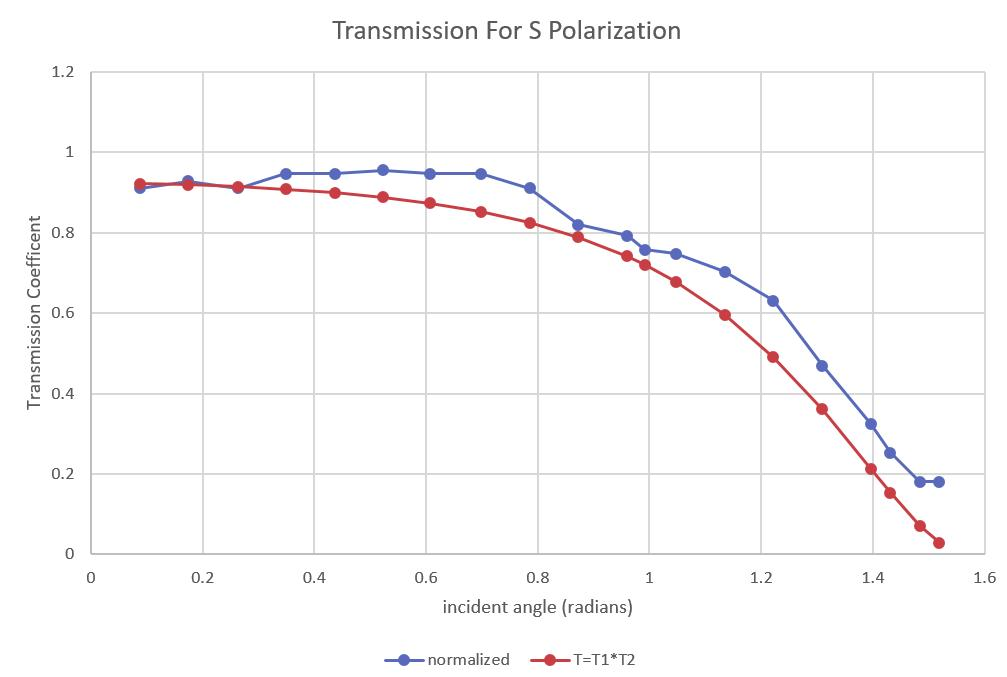
\includegraphics[width=0.75\columnwidth]{trans_s}
	\end{center}
	
\noindent For the final experiment it was necessary to consider the geometry of the sample acrylic in oder to determine the index of refraction from the measured width and apparent beam separation. The following illustration shows how this geometry was considered.\\
	\begin{center}
		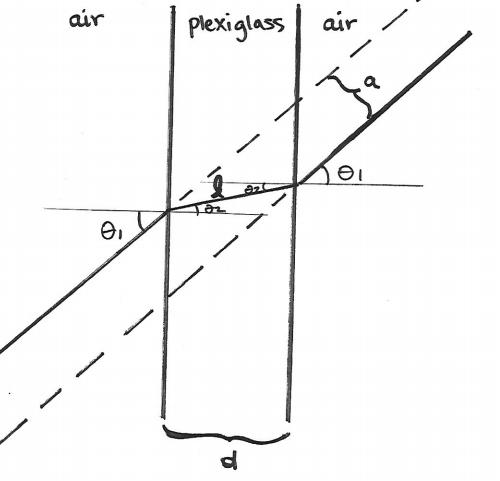
\includegraphics[scale=.35]{plexiglass}
	\end{center}
\noindent From figure 4 it is apparent that there are two triangles that can be used to solve for the index of refraction in terms of d and a. They are: \\
	\begin{center}
		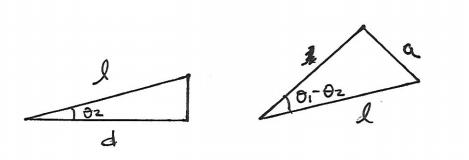
\includegraphics[scale=.35]{triangles}
	\end{center}
From these triangles and the known angle $\theta_i$ we can solve for n. 
	\begin{align*}
		\ell &= \frac{d}{\cos\theta_2} \\ 
		\ell &= \frac{a}{\sin(\theta_1-\theta_2)}
		\Rightarrow d\sin(\theta_1-\theta_2) &= a\cos(\theta_2) \\ 
		\sin\theta_1\cos\theta_2-\cos\theta_1\sin\theta_2 &= \frac{a}{d}\cos\theta_2\\ 
		\sin\theta_1-\cos\theta_1\tan\theta_2 &= \frac{a}{d} \\ 
		\Rightarrow \theta_2 &= \arctan(\tan\theta_1-a/(d\cos\theta_1)) \\ 
		\arcsin(\sin(\theta_1)/n_2) &= \sin(\arctan(\tan\theta_1-a/(d\cos\theta_1))) \\ 
		\Rightarrow n_2 &= \frac{\sin\theta_1}{\sin(\arctan(\tan\theta_1-a/(d\cos\theta_1)))} \\ 
	\end{align*}
We chose to set $\theta_i = \frac{\pi}{4}$ for simplicity. The value of a was measured to be 5.5mm and d was measured to be 17 millimeters. Thus: 
	\begin{equation}
		n_2 \approx 1.48296 
	\end{equation}

\section*{Discussion} 
As the figures show, there was phenomenal agreement for the reflection coefficients of both polarization to their theoretical counterparts with only slight deviation near the final data points. The transmission coefficients were much more difficult to take though as the thin nature of the glass slides used led to thin film diffraction becoming an appreciable concern. Particularly for the S polarization we can see how there is significant noise in the data. We tried to ameliorate this by using a card to check the intensity of the reflected light and make sure we found a maximum before reading the oscilloscope. Regardless it is still clear that the data follows the theoretical trend. Furthermore, when we calculated the index of refraction, we found 1.53 for glass (which we have been approximating in class as 1.5 this whole term) and 1.48296 for the acrylic. This is very close to the reported value of 1.490.1.492. The difference in this number is likely the result of two things: the first is that our length measurements were only precise to the millimeter, and the second is that the index of refraction can be wavelength dependent and so the wavelength we derived may vary due to the type of HeNe laser we used. \\

\noindent 
Potential sources for experimental uncertainty are largely from distance measurements that were made by hand. It is difficult to specify the accuracy of rotational stage as this was entirely controlled in software. Other than that, slight variations in the thickness of the glass and acrylic used could have an impact on the laser light. Time was a concern and knowing now about the impact of the diffraction on the transmission data, I would take more points towards the 90 degree mark as those tended to show the most variation. 

\section*{Conclusions} 
We were able to find the Brewster angle for a laser beam incident to a thin pane of glass. Using this we determined the index of refraction to be 1.53 and subsequently measured the transmission and reflection coefficients as functions of incident angle for both the S and P polarizations. Both seem to agree well with the theoretical curves despite noise due to thin film diffraction. Finally we determined the index of refraction for acrylic to be 1.48296 which is close to the literature value of 1.490. 

\section*{References} 
(1) Darlene Focht \\
(2) \url{https://en.wikipedia.org/wiki/List_of_refractive_indices}\\
(3) \url{http://physics.oregonstate.edu/~mcintyre/COURSES/ph481/LABS/Lab2.pdf}\\
(4) \textit{optics} by Eugene Hecht \\
\end{document}







































